\documentclass[12pt]{article}
\usepackage[margin=1in]{geometry}
\usepackage{relsize}
\usepackage{amssymb}
\usepackage{amsmath}
\usepackage{enumitem}
\usepackage{tikz}
\usetikzlibrary{automata,positioning}

\hyphenpenalty=10000
\setlength{\parindent}{0pt}

\newcommand\bicond{\mathrel{\leftrightarrow}}
\newcommand\bufprob{\vspace{2.0in}}
\newcommand\bufsub{\vspace{1.0in}}
\let\union\cup
\let\intersect\cap

\newenvironment{answer}{\larger[2]}{}

\begin{document}

\begin{center}
CS 441: Discrete Structures for Computer Science \\
{\smaller[1] Spring 2020} \\

\vspace {0.25in}

SOLUTION: Practice Worksheet for remaining sections
\end{center}

\vspace{0.25in}

{\smaller[1]
\textbf{Username (abc123):} \rule{1.25in}{0.4pt}
}

\begin{center}
    {\large Section 9.1}
\end{center}

\begin{enumerate} % start main problems

% PROBLEM 1 (9.1 #1 (d))

\item[1. (d)] List the ordered pairs in the relation $R$ from $A = \{ 0,1,2,3,4 \}$ to $B = \{ 0, 1, 2, 3 \}$, where $(a,b) \in R$ if and only if $a | b$. Recall that $a | b$ means that a divides b or that $b = n \times a$ for some $n \in \mathbb{Z}$ (the integers).

\begin{answer}
   The ordered pairs are:
   
   (1, 0), (1, 1), (1, 2), (1, 3), (2, 0), (2, 2), (3, 0), (3, 3), (4, 0) since in all of these pairs $a | b$.
\end{answer}

\bufprob
%


% PROBLEM 2 (9.1, #3 (b) (e))

\item[3.] For each of these relations on the set $\{ 1,2,3,4 \}$, decide whether it is reflexive, whether it is symmetric, whether it is antisymmetric, and whether it is transitive.

\begin{enumerate}
    \item[(b)] $\{ (1,1), (1,2), (2,1), (2,2), (3,3), (4,4) \}$.
    
    \begin{answer}
        Since $(a, a) \in R$ for all elements in the set, R is reflexive.

        Since $\forall (a, b) \in R, (b, a) \in R$, R is symmetric. 

        Since $(1, 2) \in R$ and $(2, 1) \in R$ but $1 \neq 2$, R is not antisymmetric.

        Since $\forall (a, b), (b, c) \in R$, $(a, c) \in R$ e.g. $(1, 2), (2, 1) \to (1, 1) \in R$, R is transitive.
    \end{answer}

    \vspace{0.2in}
    
    \item[(e)] $\{ (1,1), (2,2), (3,3), (4,4) \}$.
    
    \begin{answer}
        Since $(a, a) \in R$ for all elements in the set, R is reflexive.

        Since $\forall (a, b) \in R, (b, a) \in R$, R is symmetric.

        Since $\forall (a, b) \in R, (b, a) \in R$, and $a = b$, R is antisymmetric.

        Since $\forall (a, b), (b, c) \in R, (a, c) \in R$, here $a = b = c$, R is transitive.
    \end{answer}
    
\end{enumerate}

\bufsub


% PROBLEM 3 (9.1 #7 (a) (b))

\item[7.] Determine whether the relation R on the set of all integers is reflexive, symmetric, antisymmetric, and/or transitive, where $(x,y) \in R$ if and only if:
%
\begin{enumerate}

\item[(a)] $x \neq y$.

\begin{answer}
    R is not reflexive since for $(x, x), x \neq x$ is false. In other words, $(x, x) \notin R, \forall x \in \mathbb{Z}$.

    Given that $(x, y) \in R$, that is, $x \neq y \neq x$. In other words, $(y, x) \in R, \forall x, y \in R$. Therefore, R is symmetric.

    From the previous, proof for symmetry, it follows easily that R is not antisymmetric. If $(x, y) \in R$, then $x \neq y \neq x$, then it can't be the case that $x = y$ for antisymmetry.

    Given that $(x, y), (y, z) \in R$, then $x \neq y$ and $y \neq z$. However, consider the counterexample where x = 1, y = 2, and z = 1. Then $x \neq y, y \neq z$, but $x = z$ which means that $\exists x, y, z \in \mathbb{Z} | (x, z) \notin R$.

    Therefore, R is not transitive.
\end{answer}

\item[(b)] $xy \geq 1$.

\begin{answer}
    Given $(x, x) \in R$, then $xx \geq 1$. Consider the case when $x = 0$. Then, $xx = 0 \not \geq 1$. Therefore, since $\exists (x, x) \notin R$, R is not reflexive.

    Given $(x, y) \in R$, that is, $xy \geq 1$, then $yx \geq 1$ by commutativity. 
    
    Therefore, R is symmetric since $(x, y), (y, x) \in R$.

    Consider the case where $x = 1, y = 2$, then $xy \geq 1$ and $yx \geq 1$. $(1, 2), (2, 1) \in R$, but $x \neq y$. Thus, R is not antisymmetric.

    Given $(x, y), (y, z) \in R$, then $xy \geq 1$ and $yz \geq 1$. Therefore, $x \neq 0, y \neq 0, z \neq 0$ else the relation would not hold. 

    If $y > 0$, then $x > 0$ and $z > 0$ in order to satisfy $xy \geq 1$ and $yz \geq 1$.

    Therefore, $xz > 0 \to xz \geq 1$ and $(x, z) \in R$.

    If $y < 0$, then $x < 0$ and $z < 0$ in order to satisfy $xy \geq 1$ and $yz \geq 1$.

    Therefore, $xz > 0 \to xz \geq 1$ and $(x, z) \in R$.

    Since $(x, z) \in R$ for all cases, R is transitive.
\end{answer}

\end{enumerate}
%

\newpage


% PROBLEM 4 (9.1 #35 (a) (c))

For the following problem, let:

\begin{align*}
    R_2 &= \{ (a,b) \in \mathbb{R}^2 | a \geq b \}, \text{ the greater than or equal to relation} \\
    R_3 &= \{ (a, b) \in \mathbb{R}^2 | a < b \}, \text{ the less than relation} \\
    R_4 &= \{ (a, b) \in \mathbb{R}^2 | a \leq b \}, \text{ the less than or equal to relation} \\
    R_6 &= \{ (a, b) \in \mathbb{R}^2 | a \neq b \}, \text{ the unequal to relation} \\
\end{align*}

\item[35.] Find the following relations:

\begin{enumerate}
    \item[(a)] $R_2 \cup R_4$.
    
    \begin{answer}
        Since the domain of $R_2$ is $a \geq b$ and $R_4$ is $a \leq b$, the union is the entire range of $\mathbb{R}$. That is, the elements of the union are members of $\mathbb{R}^2$.
    \end{answer}
    
    \item[(c)] $R_3 \cap R_6$.
    
    \begin{answer}
        Since $a \neq b$ is always the case when $a < b$, and the number of values in $a < b$ is smaller than the values where $a \neq b$, the intersect is $R_3$. We take the smaller domain here since we are taking the intersection. 
    \end{answer}
    
\end{enumerate}

\newpage

\begin{center}
    {\large Sections 4.1 to 4.3}
\end{center}


% PROBLEM 5 (4.1 #13 (a) (b))

\item[13.]  What are the quotient and remainder when:

\begin{enumerate}
    \item[(a)] 19 is divided by 7?
    
    \begin{answer}
        $19 = 2 \times 7 + 5$. The quotient is 2 and remainder is 5.
    \end{answer}
    
    \vspace{0.2in}

    \item[(b)] -111 is divided by 11?
    
    \begin{answer}
        $-111 = -11 \times 11 + 10$. The quotient is -11 and the remainder is 10.
    \end{answer}
    
\end{enumerate}
\bufsub

% Problem 6 (4.1 #15 (c))

\item[15. (c)] What time does a 12-hour clock read 100 hours after it reads 6:00?

\begin{answer}
    Since the clock is based on 12 hours, we will use modulo 12. What we are trying to calculate is (100 + 6) mod 12. 
    
    Note: There is a simpler way to calculate this thanks to some tricks from Abstract Algebra (which I won't prove here). 

    (100 + 6) mod 12 can be rewritten as 100 mod 12 + 6 mod 12.

    100 mod 12 $\equiv$ 4 mod 12 (since $96 = 12 \times 8$). 

    Now, 100 mod 12 + 6 mod 12 = 4 mod 12 + 6 mod 12 = (4 + 6) mod 12 = 10 mod 12. 
    
    So the clock will read 10:00 after 100 hours.
\end{answer}
\bufsub 

% Problem 7 (4.1 #29 (a) (c))

\item[29.] Find a \emph{div} m and a \emph{mod} m when:

\begin{enumerate}
    \item[(a)] a = 228, m = 119.
    
    \begin{answer}
        $228 = 1 \times 119 + 109$.

        228 div 119 = 1.

        228 mod 119 = 109.
    \end{answer}
    
    \item[(c)] a = -10101, m = 333.
    
    \begin{answer}
        $-10101 = -31 \times 333 + 222$

        -10101 div 333 = -31.

        -10101 mod 333 = 222.
    \end{answer}
    
\end{enumerate}
\bufsub

% Problem 8 (4.1 #35 (b) (c))

\item[35.] Decide whether each of these integers is congruent to 5 modulo 17.

\begin{enumerate}
    \item[(b)] 103
    
    \begin{answer}
        \begin{align*}
            103 - 17 = 86 \\
            86 - 17 = 69 \\
            69 - 17 = 52 \\
            52 - 17 = 35 \\
            35 - 17 = 18 \\
            18 - 17 = 1 \\
        \end{align*}

        $103 \not \equiv 5$ mod 17.
    \end{answer}
    
    \item[(c)] -29
    
    \begin{answer}
        \begin{align*}
            -29 + 17 = -12 \\
            -12 + 17 = 5 \\
        \end{align*}

        $-29 \equiv 5$ mod 17.
    \end{answer}
    
\end{enumerate}
\newpage

%Problem 9 (4.2 #1 (a) (b))

\item[1.] Convert the decimal expansion of each the these integers to a binary expansion.

\begin{enumerate}
    \item[(a)] 231
    
    Standard Method:

    \begin{align*}
        231 - 128 = 103 [128 = 2^7]\\
        103 - 64 = 39 [64 = 2^6]\\
        39 - 32 = 7 [32 = 2^5]\\
        7 - 4 = 3 [4 = 2^2]\\
        3 - 2 = 1 [2 = 2^1]\\
        1 - 1 = 0 [1 = 2^0]\\
    \end{align*}

    1110 0111 is the binary expansion of 231.

    Faster Method:

    Divide the value by 2 until zero, if it's even, write a 0, if it's not, round down and write a 1.

    $231 \to_{1} 115 \to_{1} 57 \to_{1} 28 \to_{0} 14 \to_{0} 7 \to_{1} 3 \to_{1} 1 \to_{1} 0$.

    Write the arrow values backwards and you'll have the binary expansion.

    1110 0111 is the binary expansion of 231.
    
    \item[(b)] 4532
    
    Faster Method:

    $4532 \to_{0} 2266 \to_{0} 1133 \to_{1} 566 \to_{0} 283 \to_{1} 141 \to_{1} 70 \to_{0} 35 \to_{1} 17 \to_{1} 8 \to_{0} 4 \to_{0} 2 \to_{0} 1 \to_{1} 0$. 

    Write backwards:

    1 0001 1011 0100 is the binary expansion.
    
\end{enumerate}
\bufsub

%Problem 10 (4.2 #6 (a))

\item[6. (a)] Convert the binary expansion of (1111 0111$)_{2}$ to an octal expansion.

\begin{answer}
    Split the binary expansion into groups of three.

    011 110 111, now each of these can be converted.

    111 = 7, 110 = 6, 011 = 3

    The octal expansion is $(367)_8$.
\end{answer}
\bufsub

%Problem 11 (4.2 #6 (c))

\item[6. (c)] Convert the binary expansion of (111 0111 0111 0111$)_2$ to a hexadecimal expansion.

\begin{answer}
    Split the binary expansion into groups of four.

    0111 0111 0111 0111, now each of these can be converted.

    $(7777)_{16}$ is the hexadecimal expansion.
\end{answer}
\bufsub

%Problem 12 (4.3 #3 (a) (b))

\item[3.] Find the prime factorization of each of these integers.

\begin{enumerate}
    \item[(a)] 88
    
    \begin{answer}
        $88 = 11 \times 8 = 11 \times 4 \times 2 = 11 \times 2^3$.
    \end{answer}
    
    \vspace{0.2in}

    \item[(b)] 126
    
    \begin{answer}
        $126 = 63 \times 2 = 21 \times 3 \times 2 = 7 \times 3 \times 3 \times 2 = 7 \times 3^2 \times 2$.
    \end{answer}
    
\end{enumerate}
\bufsub

%Problem 13 (4.3 #15)

\item[15.] Which positive integers less than 30 are relatively prime to 30?

\begin{answer}
    The prime factors of 30 are 2, 3, 5. These primes and the multiples of them less than 30 are coprime with 30 (i.e. not relatively prime).

    This leaves:

    7, 11, 13, 17, 19, 23, 29 as the integers less than 30 that are relatively prime to 30.
\end{answer}
\newpage

%Problem 14 (4.3 #18)

\item[18.] We call a positive integer \emph{perfect} if it equals the sum of its positive divisors other than itself. Show that 496 is perfect.

\begin{answer}
    Divisors of are:

    1, 2, 4, 8, 16, 31, 62, 124, 248, 496 (I obtained from Wolfram using the Factor[ ] command).

    Check:

    1 + 2 + 4 + 8 + 16 + 31 + 62 + 124 + 248 = 496

    Therefore, 496 is perfect.
\end{answer}
\bufsub

%Problem 15 (4.3 #24)

\item[24.] Find gcd(100, 125) and lcm(100, 125) and verify that gcd(100, 125) $\times$ lcm(100, 125) = $100 \times 125$.

\begin{answer}
    $100 = 10^2 = (2 \times 5)^2 = 2^2 \times 5^2$

    $125 = 5^3$.

    $gcd(100, 125) = 5^2$.

    $lcm(100, 125) = 2^2 \times 5^3$.

    Verify:

    gcd(100, 125) lcm(100, 125) = $5^2 \times 5^3 \times 2^2 =2^2 \times 5^5 = 12500$

    $100 \times 125$ = 12500.
\end{answer}
\vspace{0.2in}

\newpage
%Problem 16 (4.3 #33 (d))

\item[33.] Use the Euclidean Algorithm to find gcd(12345, 54321).

\begin{answer}
    \begin{align*}
        54321 = 4 \times 12345 + 4941 \\
        12345 = 2 \times 4941 + 2463 \\
        4941 = 2 \times 2463 + 15 \\
        2463 = 164 \times 15 + 3 \\
        15 = 5 \times 3 + 0 \\
    \end{align*}

    gcd(12345, 54321) = 3.
\end{answer}

\newpage

\begin{center}
    {\large Section 10.1}
\end{center}

%Problem 17 (10.1 #3)

\item[3.] Determine whether the graph shown has directed or undirected edges, whether it has multiple edges, and whether it has one or more loops. Use your answers to determine the type of graph. (Refer to Table 1 on page 676 of the textbook).

\hspace{50.0mm}
%Use tikzpicture to make a visual representation of the graph
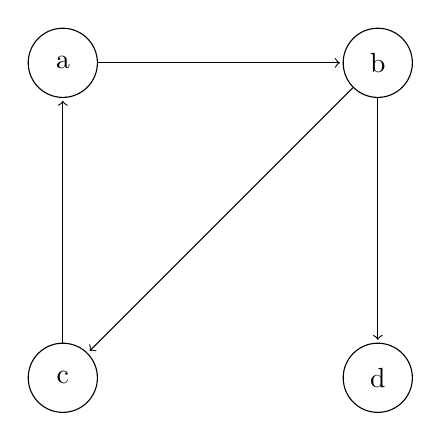
\begin{tikzpicture}[shorten >=1pt, node distance=4cm, on grid, auto]
    \node[state] (0) {a};
    \node[state] (1) [right=of 0] {b};
    \node[state] (2) [below=of 0] {c};
    \node[state] (3) [below=of 1] {d};
    \path[->]
     (0) edge				node {} (1)
     (2) edge               node {} (0)
     (1) edge				node {} (2)
     (1) edge				node {} (3);
\end{tikzpicture}

\begin{answer}
    The graph shown above has directed edges due to the arrows on each edge specifying a direction. This graph has multiple edges i.e. more than one edge and there are no loops, edges that go to the node they originated from or the ability to start at a vertex and return to it without reusing an edge, in this graph.
\end{answer}
\bufsub

%Problem 18 (10.1 #5)

\item[5.] Determine whether the graph shown has directed or undirected edges, whether it has multiple edges, and whether it has one or more loops. Use your answers to determine the type of graph. (Refer to Table 1 on page 676 of the textbook).

\hspace{42.0mm}
%Use tikzpicture to make a visual representation of the graph
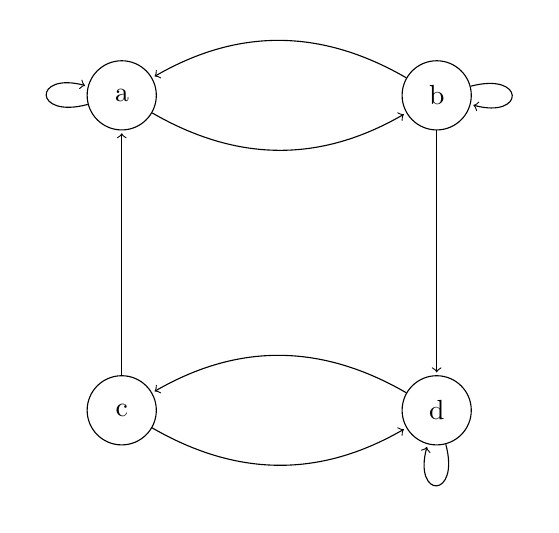
\begin{tikzpicture}[shorten >=1pt, node distance=4cm, on grid, auto]
    \node[state] (0) {a};
    \node[state] (1) [right=of 0] {b};
    \node[state] (2) [below=of 0] {c};
    \node[state] (3) [below=of 1] {d};
    \path[->]
     (0) edge [bend right]	node {} (1)
     (1) edge [bend right]  node {} (0)
     (2) edge               node {} (0)
     (3) edge [bend right]	node {} (2)
     (2) edge [bend right]  node {} (3)
     (1) edge				node {} (3)
     (0) edge [loop left]   node {} (0)
     (1) edge [loop right]  node {} (1)
     (3) edge [loop below]  node {} (3);
\end{tikzpicture}

\vfill

\begin{answer}
    This graph also has directed edges due to the arrows on each edge specifying the direction. This graph contains several edges and there are several loops in this graph. 
\end{answer}

\end{enumerate} % end main problems

\end{document}

